% =============================================================================
%  Compte rendu de TP - Chaîne de transmission numérique (Matlab/Simulink)
%  ENSIM 5A ASTRE - Théorie de l'information et du codage - 2026-2027
%  Compilation : pdfLaTeX (Overleaf : Menu > Compiler = pdfLaTeX)
%  Les images sont dans le sous-dossier figures/ (régénérées par matlab/run_all.m)
% =============================================================================
\documentclass[10pt,a4paper]{article}

% ---------- Langue et police ----------
\usepackage[utf8]{inputenc}
\usepackage[T1]{fontenc}
\usepackage[french]{babel}
\usepackage{lmodern}
\usepackage{microtype}
\usepackage{icomma}                 % virgule décimale en mode maths : $0,36$

% ---------- Mise en page ----------
\usepackage[a4paper,top=17mm,bottom=18mm,left=17mm,right=17mm,headsep=5mm]{geometry}
\usepackage{fancyhdr}
\usepackage{titlesec}
\usepackage{enumitem}
\setlength{\parindent}{0pt}
\setlength{\parskip}{3pt plus 1pt}
\setlist{nosep,leftmargin=*}

% ---------- Maths, figures, tableaux ----------
\usepackage{amsmath,amssymb}
\usepackage{graphicx}
\graphicspath{{figures/}}
\usepackage{caption}
\usepackage{subcaption}
\usepackage{booktabs}
\usepackage{array}
\usepackage{xcolor}
\usepackage{float}
\usepackage[hidelinks]{hyperref}

% ---------- Couleurs et styles ----------
\definecolor{bleu}{RGB}{31,78,121}
\definecolor{orange}{RGB}{197,90,17}
\hypersetup{colorlinks=true,linkcolor=bleu,urlcolor=orange,citecolor=bleu}

\titleformat{\section}{\large\bfseries\sffamily\color{bleu}}{\thesection.}{0.5em}{}[\vspace{-4pt}{\color{bleu}\rule{\linewidth}{0.8pt}}]
\titleformat{\subsection}{\normalsize\bfseries\sffamily\color{bleu}}{\thesubsection}{0.5em}{}
\titlespacing*{\section}{0pt}{9pt}{4pt}
\titlespacing*{\subsection}{0pt}{6pt}{2pt}

\captionsetup{font=small,labelfont={bf,color=bleu},labelsep=endash,skip=3pt}
\captionsetup[sub]{font=footnotesize}
\setlength{\textfloatsep}{8pt plus 2pt minus 2pt}
\setlength{\floatsep}{6pt plus 2pt minus 2pt}
\setlength{\intextsep}{6pt plus 2pt minus 2pt}
\renewcommand{\arraystretch}{1.15}

\pagestyle{fancy}
\fancyhf{}
\fancyhead[R]{\footnotesize\sffamily\color{gray} Chaîne de transmission numérique --- B.~KONTIEBO}
\fancyfoot[C]{\footnotesize\sffamily\thepage}
\renewcommand{\headrulewidth}{0pt}

% ---------- Raccourcis ----------
\newcommand{\EbNo}{E_b/N_0}
\newcommand{\TEB}{\mathrm{TEB}}
\newcommand{\code}[1]{\texttt{\small #1}}
\newcommand{\bloc}[1]{\textit{#1}}

\begin{document}

% =============================================================================
%  Page de garde
% =============================================================================
\newgeometry{top=0mm,bottom=15mm,left=0mm,right=0mm,nohead,nofoot}
\begin{titlepage}
\sffamily
\setlength{\fboxsep}{0pt}
% ----- Bandeau supérieur -----
\noindent\colorbox{bleu}{%
  \parbox[c][38mm][c]{\paperwidth}{%
    \hspace*{22mm}\parbox{\dimexpr\paperwidth-44mm}{%
      \color{white}
      % Logo de l'école (optionnel) : déposer logo.png dans figures/ et décommenter
      % \includegraphics[height=18mm]{logo.png}\hfill
      {\LARGE\bfseries ENSIM}\\[3pt]
      {\large École Nationale Supérieure d'Ingénieurs du Mans}\\[2pt]
      {\normalsize Le Mans Université --- 5\textsuperscript{e} année, option ASTRE}
    }}}
\par
{\color{orange}\rule{\paperwidth}{2.5mm}}

\vspace{14mm}
\begin{center}
\begin{minipage}{0.8\paperwidth}
  \centering
  {\large\color{gray} Théorie de l'information et du codage}\\[4pt]
  {\large\color{gray} Compte rendu de travaux pratiques}\\[10mm]

  {\color{bleu}\rule{\linewidth}{1.2pt}}\\[6mm]
  {\fontsize{24}{30}\selectfont\bfseries\color{bleu}
    Modélisation et simulation\\[2mm]
    d'une chaîne de transmission numérique\\[2mm]
    en bande de base\par}
  \vspace{5mm}
  {\Large sous Matlab/Simulink}\\[5mm]
  {\color{bleu}\rule{\linewidth}{1.2pt}}\\[9mm]

  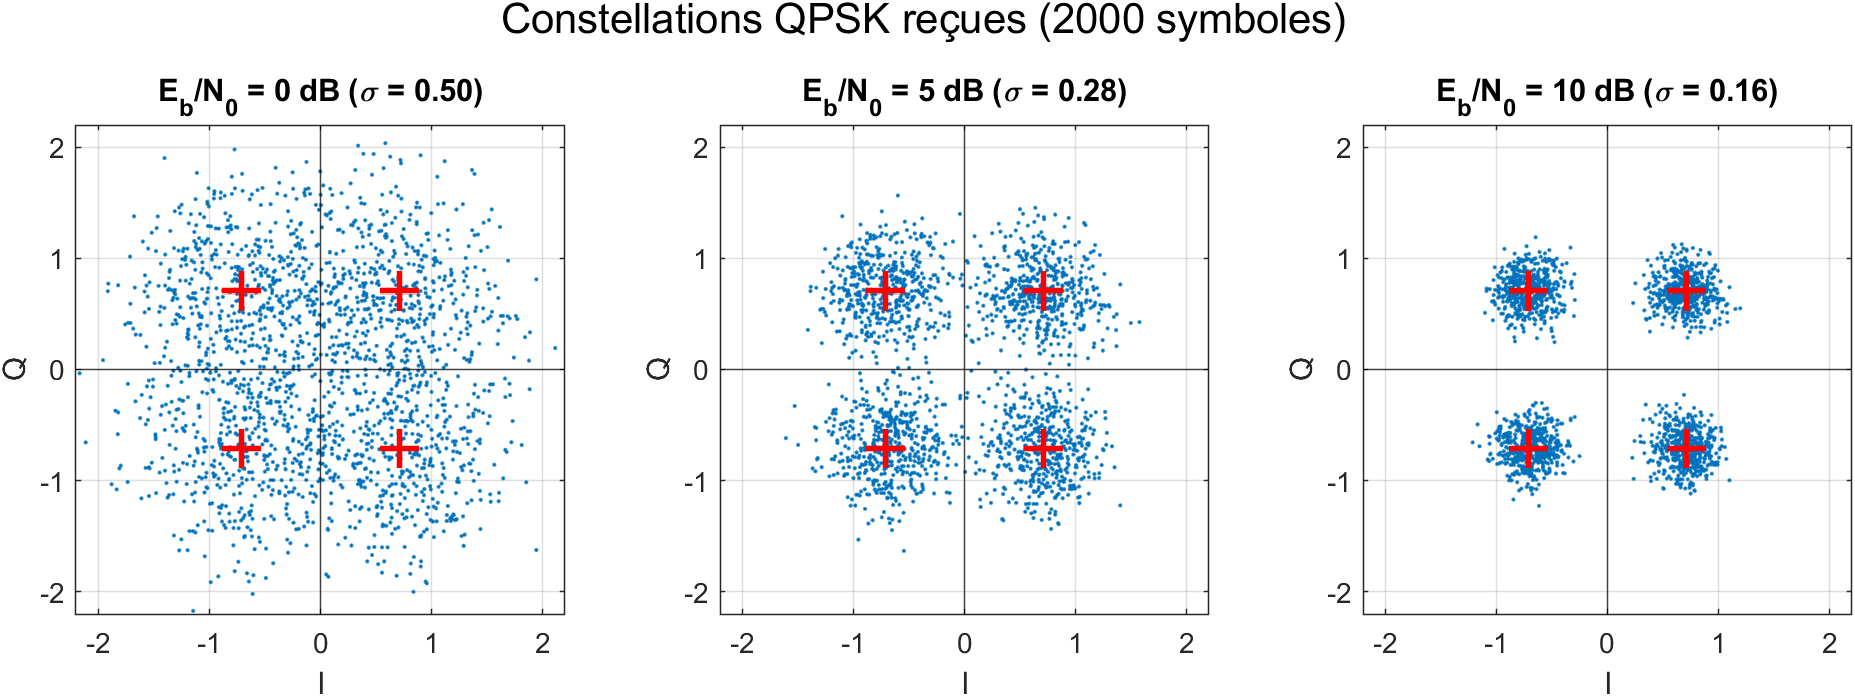
\includegraphics[width=0.92\linewidth]{partie5_qpsk_1.png}\\[2mm]
  {\small\itshape\color{gray} Constellations QPSK reçues à $E_b/N_0$ = 0, 5 et 10~dB}\\[11mm]

  \begin{tabular}{@{}r@{\hspace{6mm}}l@{}}
    \color{gray}Réalisé par   & {\Large\bfseries Bénéwindé KONTIEBO} \\[4mm]
    % \color{gray}Encadré par & Nom de l'enseignant \\[4mm]
    \color{gray}Année         & 2026 -- 2027 \\[4mm]
    \color{gray}Code source   & \url{https://github.com/fkontiebo/TP-communication-numerique}
  \end{tabular}
\end{minipage}
\end{center}

\vfill
\begin{center}
  {\color{bleu}\rule{0.8\paperwidth}{0.6pt}}\\[3mm]
  {\small\color{gray} Codage de source \;·\; Chaîne de base \;·\; Codage de canal (Hamming) \;·\; Modulation QPSK \;·\; Mise en forme RRC}
\end{center}
\end{titlepage}
\restoregeometry
\setcounter{page}{1}

% =============================================================================
\section{Introduction}
% =============================================================================
L'objectif de ce TP est de construire, bloc par bloc, une chaîne de transmission numérique complète et de mesurer, à chaque étape, ce qu'apporte le bloc ajouté. On commence par le \textbf{codage de source}, étudié seul (entropie, Huffman, Lempel-Ziv), puis on modélise une \textbf{chaîne de base} source--canal--décision, à laquelle on ajoute successivement un \textbf{code correcteur} de Hamming (7,4), une \textbf{modulation QPSK} et des \textbf{filtres de mise en forme} en racine de cosinus surélevé. Les performances sont évaluées par le taux d'erreur binaire (TEB) en fonction de $\EbNo$, systématiquement confronté à la théorie et aux limites de Shannon, ainsi qu'en termes de débit et d'occupation spectrale.

\textbf{Méthode et reproductibilité.} Le codage de source est réalisé par des fonctions Matlab ; les parties 3 à 6 sous Simulink (solveur discret à pas fixe $T_e=T_b/L$, sous-systèmes, changements de rythme par \bloc{Buffer/Unbuffer/Rate Transition}). Tous les paramètres sont regroupés dans \code{Parametres.m}. Chaque courbe de TEB est pilotée par une fonction commune \code{trace\_TEB.m} qui, pour chaque $\EbNo$, calcule $\sigma^2 = N_0/(2T_e)$, lance \code{sim} et arrête la mesure après \textbf{100 erreurs ou $10^6$ bits}, avec un intervalle de confiance à 95\,\% $\hat p \pm 1,96\sqrt{\hat p(1-\hat p)/N}$. Les retards introduits par les blocs sont \textbf{recherchés automatiquement} (simulation sans bruit : seul le bon retard donne 0 erreur). Le script \code{run\_all.m} rejoue l'intégralité du TP et régénère, à l'identique, toutes les figures de ce rapport ; les sorties numériques complètes sont dans le dossier \code{resultats/} du dépôt.

\begin{table}[H]
\centering\small
\begin{tabular}{ccccccccc}
\toprule
$p_1$ & $p_{1,\mathrm{ext}}$ & $p_e$ (CBS) & $a$ (uniforme) & $\sigma$ (gaussien) & $L$ & $\alpha$ (RRC) & $\beta,\ \tau$ (écho) & graine \\
\midrule
0,36 & 0,11 & 0,068 & 1,64 & 0,88 & 16 & 0,35 & 0,23 ; $2T$ & 33 \\
\bottomrule
\end{tabular}
\caption{Paramètres personnels (tirés une fois puis figés dans \code{mes\_parametres.mat}). Conventions : $T_b=1$, $A=1$, $E_b=A^2T_b$.}
\label{tab:param}
\end{table}

% =============================================================================
\section{Codage de source}
% =============================================================================
\subsection{Source binaire et entropie}
La source \code{source(N,p1)} tire $u\sim\mathcal U[0,1]$ et émet 1 si $u<p_1$ (même principe sous Simulink avec le bloc \bloc{Uniform Random Number} cadencé à $T_b$). Sur $10^5$ bits, la fréquence empirique des 1 vaut \textbf{0,3576}, dans l'intervalle de confiance à 95\,\% $[0,3570 ; 0,3630]$ autour de $p_1=0,36$. L'entropie vaut $H(0,36) = 0,9427$ bit/symbole : à 1 bit/s, la source ne délivre que \textbf{0,943 bit/s d'information}, soit une redondance de 5,7\,\%. Une source aussi peu déséquilibrée est donc déjà presque incompressible.

\subsection{Entropie d'un texte et code de Huffman}
Le texte choisi est \textbf{\textit{Candide ou l'Optimisme} de Voltaire} (édition Beuchot, Wikisource), nettoyé de ses en-têtes : \textbf{201\,499 caractères} UTF-8, alphabet de \textbf{$M = 97$ symboles}. L'entropie d'ordre 0 vaut \textbf{$H = 4,557$ bit/caractère} ; un code de longueur fixe nécessite $\lceil\log_2 97\rceil = 7$ bits, d'où une redondance de 43\,\% par rapport à un codage sur 8 bits (35\,\% par rapport à 7 bits).

La fonction \code{huffman\_code} fusionne itérativement les deux nœuds les moins probables ; chaque nœud mémorise la liste de ses feuilles, auxquelles on préfixe «~0~» ou «~1~». Elle est validée sur $(0,4 ; 0,2 ; 0,2 ; 0,1 ; 0,1)$ : code préfixe, somme de Kraft égale à 1, longueur moyenne \textbf{2,2 bits}, identique à \code{huffmandict}. Sur le texte, on obtient $\bar L = 4,579$ bit/caractère, soit une \textbf{efficacité $H/\bar L = 99,5\,\%$}, et $H \le \bar L < H+1$ est bien vérifié (mots de 3 à 18 bits). Le décodeur parcourt l'arbre reconstruit à partir des mots de code (décodage instantané grâce à la propriété préfixe) : le texte est restitué \textbf{sans aucune erreur}, avec un taux de compression de \textbf{0,572} par rapport à 8 bits/caractère (gain de 42,8\,\%).

\textbf{Coût de la table.} Le décodeur doit connaître le code : transmettre, pour chaque symbole, son code Unicode, la longueur de son mot et le mot lui-même coûte \textbf{2\,821 bits} (1\,843 bits seulement avec un code de Huffman canonique, où les longueurs suffisent). Cela ne représente que 0,31\,\% du message codé ici ; la table devient négligeable ($<1\,\%$) dès que le texte dépasse environ \textbf{62\,000 caractères}.

\subsection{Extension de la source}
Pour une source binaire, Huffman symbole par symbole ne fait pas mieux qu'1 bit/bit. On code donc des blocs de $k$ bits (la $k$-ième extension, $2^k$ symboles de probabilité $p^w(1-p)^{k-w}$) d'une source très déséquilibrée $p_{1,\mathrm{ext}} = 0,11$, d'entropie $H = 0,500$ bit. La figure~\ref{fig:ext} (gauche) montre que $\bar L_k/k$ passe de 1 ($k=1$, efficacité 50\,\%) à \textbf{0,518 pour $k=4$}, puis 0,501 pour $k=6$ (efficacité 99,8\,\%), toujours entre $H$ et $H+1/k$ ; les valeurs mesurées en codant $10^5$ bits coïncident avec la théorie à $10^{-3}$ près. C'est le \textbf{premier théorème de Shannon} : pour une source sans mémoire, on peut coder avec un nombre moyen de bits par symbole aussi proche que voulu de $H$, mais jamais en dessous. Le prix à payer est la taille du dictionnaire ($2^k$ mots, jusqu'à 29 bits pour $k=10$), le délai de codage (on attend $k$ bits) et la sensibilité aux erreurs de transmission. La décroissance n'est d'ailleurs pas monotone ($\bar L_7/7 > \bar L_6/6$) : seule la borne $H+1/k$ l'est.

\begin{figure}[!htb]
\centering
\begin{subfigure}{0.49\linewidth}\centering
  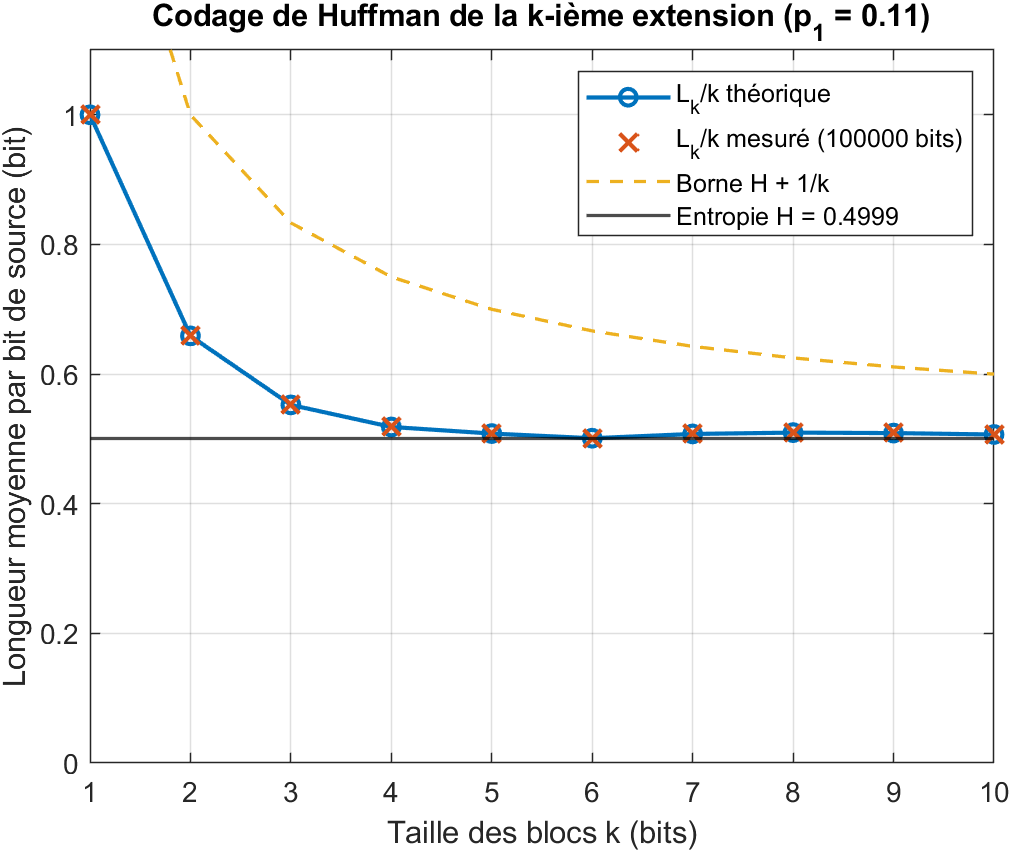
\includegraphics[width=\linewidth]{partie2_3_1.png}
  \caption{Huffman de la $k$-ième extension.}
\end{subfigure}\hfill
\begin{subfigure}{0.49\linewidth}\centering
  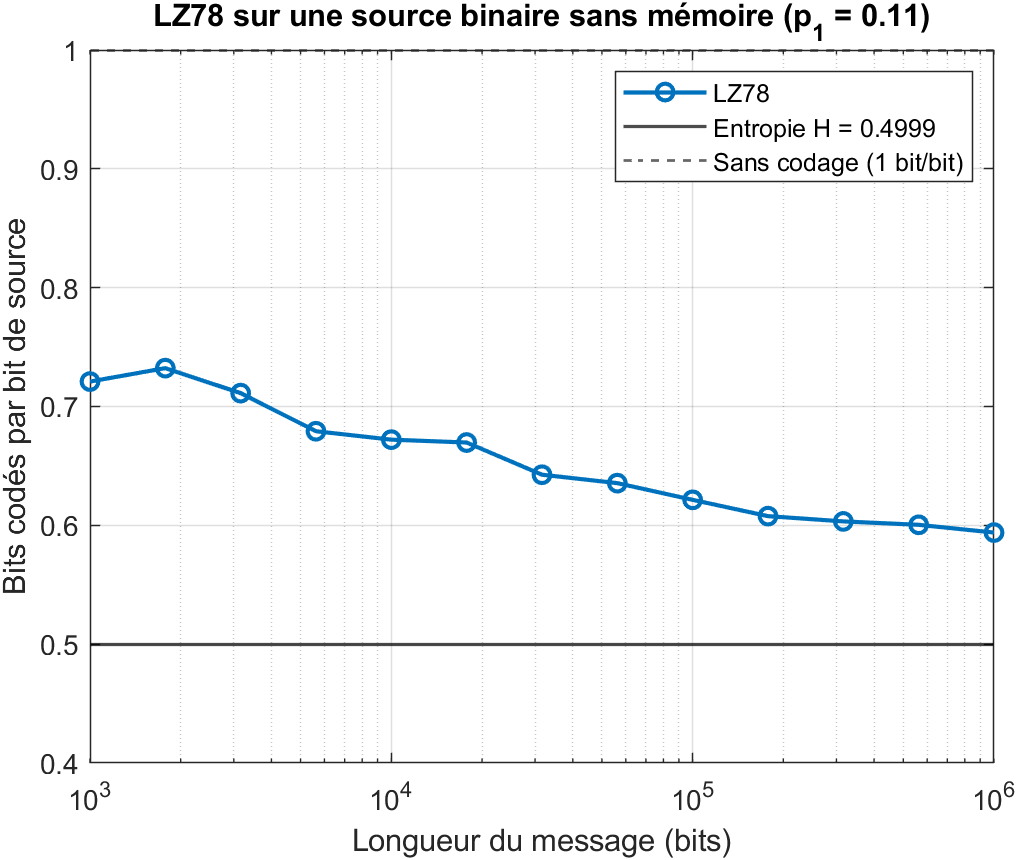
\includegraphics[width=\linewidth]{partie2_5_1.png}
  \caption{LZ78 en fonction de la longueur du message.}
\end{subfigure}
\caption{Codage d'une source binaire très déséquilibrée ($p_1 = 0,11$, $H = 0,500$ bit).}
\label{fig:ext}
\end{figure}

\subsection{Sources avec mémoire et compresseurs réels}
\begin{table}[!htb]
\centering\small
\begin{tabular}{lcccccccc}
\toprule
bit/caractère & Long. fixe & $H_0$ & Huffman & $H(X_1X_2)/2$ & LZ78 & gzip & bzip2 & 7z (LZMA) \\
\midrule
Texte complet (201\,499 car.) & 7 & 4,557 & 4,579 & 4,011 & 4,139 & 3,158 & \textbf{2,513} & 2,753 \\
5\,000 premiers caractères   & 7 & 4,971 & 5,007 & 4,071 & 5,275 & 3,819 & \textbf{3,603} & 3,968 \\
\bottomrule
\end{tabular}
\caption{Comparaison des méthodes de codage (la table de Huffman n'est pas comptée ; les compresseurs incluent leurs en-têtes).}
\label{tab:compr}
\end{table}

L'entropie par caractère estimée sur les paires, $H(X_1X_2)/2 = 4,01$ bits, est nettement inférieure à $H_0$ : le texte a de la \textbf{mémoire} ($H(X_2|X_1) = 3,46$ bits ; seules 1\,545 paires sur 9\,409 possibles apparaissent). Huffman, qui ne voit que les fréquences, ne peut pas descendre sous $H_0$, alors que les compresseurs exploitent les répétitions de mots et de séquences longues : gzip (LZ77 + Huffman) atteint 3,16 bits et bzip2 (transformée de Burrows-Wheeler) \textbf{2,51 bits/caractère}, sous $H_0$ et même sous $H(X_1X_2)/2$, car ils captent des dépendances bien plus longues que deux caractères. Sur 5\,000 caractères, tous les taux se dégradent : $H_0$ et $H(X_1X_2)/2$ sont mal estimés (et sous-estimés pour les paires : 702 paires observées), le dictionnaire des méthodes adaptatives n'a pas le temps de se remplir et les en-têtes pèsent davantage.

\textbf{Sortie du codeur.} En sortie de Huffman, la proportion de 1 vaut 0,532 et l'entropie des paires de bits 0,997 bit/bit (paires 00 à 11 de probabilités 0,21 à 0,28) : un bon codeur de source produit des \textbf{bits quasi indépendants et équiprobables}, puisque toute redondance restante serait encore compressible. C'est ce qui justifie de modéliser la source de la chaîne de transmission par des bits i.i.d.\ équiprobables dans toute la suite.

\subsection{Complément : codage de Lempel-Ziv 78}
Le codeur LZ78 utilise un dictionnaire en arbre (\textit{trie}) pour trouver en $O(1)$ par symbole la plus longue phrase connue ; il est validé sur l'exemple de l'énoncé (\code{(0,A)(0,B)(1,A)(2,A)(4,A)(4,B)}, 17 bits) et sur $10^4$ symboles aléatoires. Sur le texte complet, il atteint \textbf{4,14 bit/caractère, sous $H_0$} sans connaître aucune statistique, mais 5,28 bits sur 5\,000 caractères. Sur la source binaire $p_{1,\mathrm{ext}}$ (fig.~\ref{fig:ext}b), le taux décroît lentement de 0,72 à \textbf{0,594 bit/bit pour $10^6$ bits}, encore 19\,\% au-dessus de l'entropie : le code est \textbf{universel} (il converge vers $H$ pour toute source stationnaire), mais sa convergence est très lente (l'écart à $H$ ne décroît qu'en $\log\log N/\log N$). Il n'est intéressant que pour des fichiers longs, et c'est pourquoi les compresseurs réels combinent dictionnaire et codage entropique.

% =============================================================================
\section{Chaîne de transmission de base}
% =============================================================================
\subsection{Canal binaire symétrique}
Le CBS inverse chaque bit avec la probabilité $p_e = 0,068$ (XOR avec une séquence de Bernoulli). Sur $10^6$ bits, le TEB mesuré est \textbf{0,06782}, IC 95\,\% $[0,06733 ; 0,06832]$, compatible avec $p_e$. Sa capacité vaut $C = 1 - H(0,068) = \mathbf{0,642}$ \textbf{bit/utilisation}. Le rendement du code de Hamming, $R = 4/7 = 0,571 < C$ : le théorème de Shannon garantit l'existence de codes de ce rendement permettant une transmission fiable sur ce canal (c'est possible tant que $p_e < 0,0876$). Pour $p_e = 0,5$, $C = 0$ : la sortie est indépendante de l'entrée et aucune information ne passe.

\subsection{Bruit uniforme et bruit gaussien : seuil optimal}
\textbf{Bruit uniforme sur $[-a,a]$.} Les vraisemblances $f(r|0)$ et $f(r|1)$ sont des portes de hauteur $1/(2a)$ centrées sur $\mp A$. Si $a \le A$, les supports sont disjoints et aucune erreur n'est possible. Ici $a = 1,64 > A$ : elles se recouvrent sur $[A-a,\,a-A] = [-0,64 ; 0,64]$, où elles sont \textbf{égales} ; la règle MAP ne compare donc que $p_0$ et $p_1$. Comme $p_0 = 0,64 > p_1$, on décide 0 sur toute la zone : \textbf{seuil optimal $s^* = a - A = 0,64$} (si $p_0 = p_1$, tout seuil de la zone serait optimal : il n'est pas unique). Pour $|s| \le a-A$ :
\[
  P_e(s) = p_0\,\frac{a-A-s}{2a} + p_1\,\frac{s-A+a}{2a},
\]
fonction affine de pente $(p_1 - p_0)/(2a) < 0$, minimale au bord : $P_e(0) = 0,195$ et $P_e(s^*) = 0,140$. La simulation (fig.~\ref{fig:seuils}a, $10^6$ bits par seuil) suit exactement cette droite.

\textbf{Bruit gaussien.} L'égalité $p_0 f(s|0) = p_1 f(s|1)$ donne $s^* = \frac{\sigma^2}{2A}\ln\frac{p_0}{p_1}$ et $P_e(s) = p_0\,Q\!\left(\frac{s+A}{\sigma}\right) + p_1\,Q\!\left(\frac{A-s}{\sigma}\right)$. Avec $\sigma = 0,88$ : \textbf{$s^* = 0,223$}, $P_e(s^*) = 0,1206$ contre $0,1279$ pour $s=0$, soit un gain de 5,7\,\% ; la simulation donne $0,1208 \pm 0,0006$ et le meilleur seuil testé, 0,225, confirme le calcul (fig.~\ref{fig:seuils}b).

\textbf{Comparaison.} Le seuil gaussien dépend de $\sigma$ car le rapport de vraisemblance varie continûment avec $r$ : plus le bruit est fort, plus l'a priori pèse et plus le seuil s'éloigne de 0. Dans le cas uniforme, le rapport de vraisemblance vaut 0, 1 ou $\infty$ : seule compte la \textbf{position} de la zone de recouvrement, pas la forme fine de la densité. Le bruit uniforme est borné, donc «~moins dangereux~» loin des symboles, mais il est ici plus fort ($\sigma_u = a/\sqrt3 = 0,95$).

\begin{figure}[!htb]
\centering
\begin{subfigure}{0.49\linewidth}\centering
  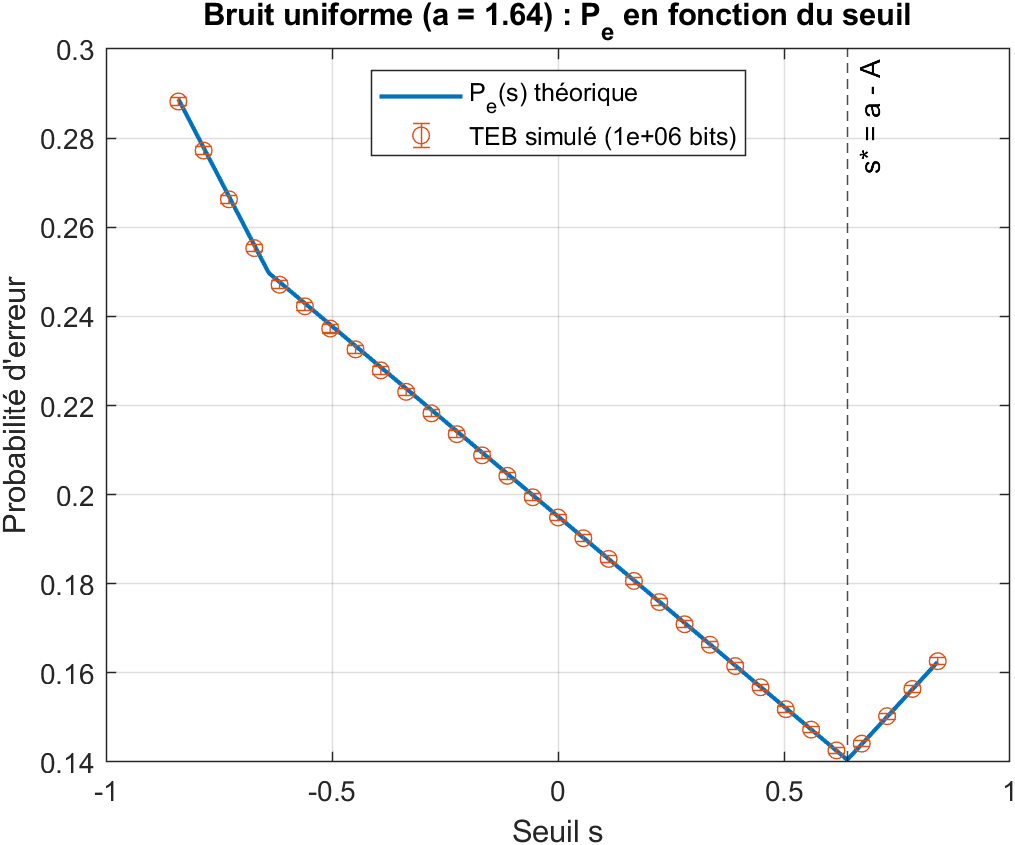
\includegraphics[width=\linewidth]{partie3_canaux_3.png}
  \caption{Bruit uniforme : $P_e(s)$ affine par morceaux.}
\end{subfigure}\hfill
\begin{subfigure}{0.49\linewidth}\centering
  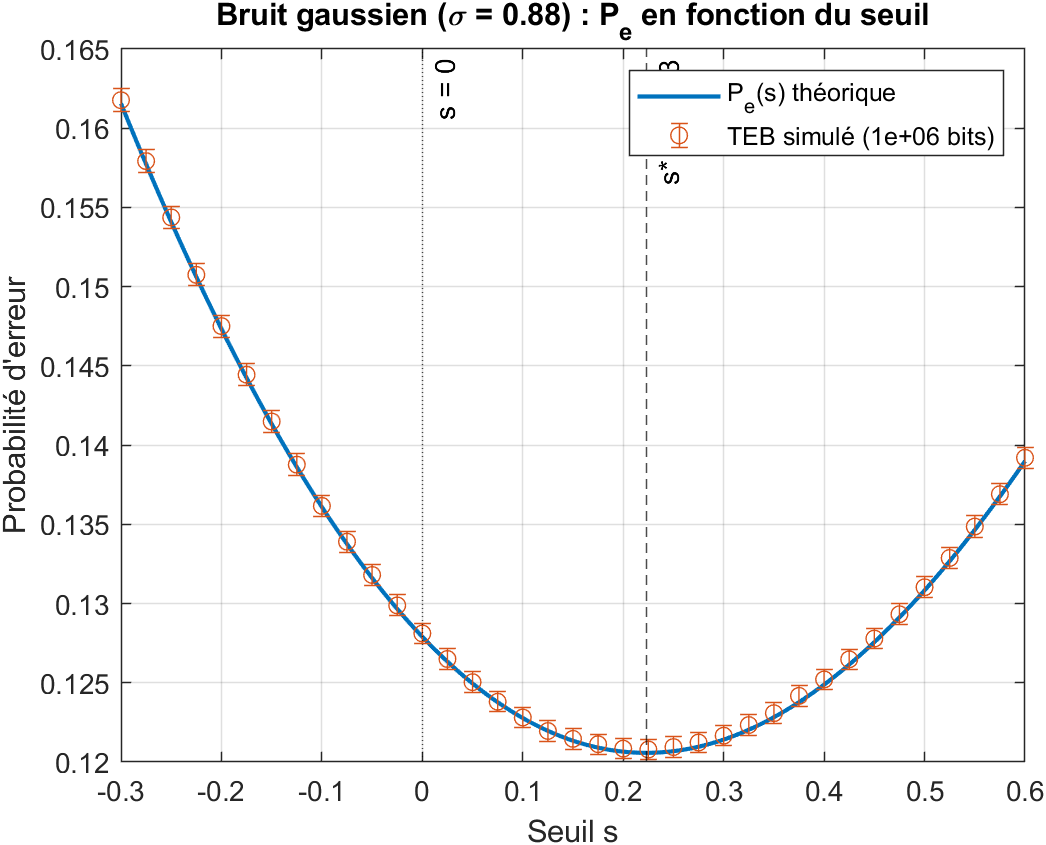
\includegraphics[width=\linewidth]{partie3_canaux_4.png}
  \caption{Bruit gaussien : minimum en $s^* = 0,223$.}
\end{subfigure}
\caption{Probabilité d'erreur en fonction du seuil : théorie et simulation ($10^6$ bits, IC 95\,\%).}
\label{fig:seuils}
\end{figure}

\subsection{Détecteur optimal sous Simulink}
Le modèle \code{chaine\_P3.slx} répète chaque niveau $\pm A$ sur $L = 16$ échantillons ($T_e = 1/16$), ajoute un bruit gaussien de variance $\sigma^2 = N_0/(2T_e) = N_0L/2$ calculée dans le script, puis applique l'intégrateur remis à zéro, réalisé par un filtre FIR de coefficients $1/L$ (moyenne glissante sur un bit), échantillonné à $T_b$ et suivi d'un comparateur à seuil nul. Le retard de la voie de référence, trouvé sans bruit, vaut \textbf{$D = 2$ bits}.

La sortie de l'intégrateur vaut $z_k = \pm A + \frac1L\sum_i n_{kL+i}$, de variance $\sigma^2/L = N_0/(2T_b)$, d'où
\[
  \TEB = Q\!\left(\frac{A}{\sqrt{N_0/2T_b}}\right) = Q\!\left(\sqrt{2E_b/N_0}\right).
\]
L'intégrateur est bien un \textbf{filtre adapté} : sa réponse (porte de durée $T_b$) est la forme d'onde émise retournée, ce qui maximise le rapport signal à bruit à l'instant de décision. La figure~\ref{fig:p3} montre l'accord entre simulation et théorie sur toute la plage 0--9~dB. Sans intégration (un seul échantillon au milieu du bit), la variance du bruit reste $\sigma^2$ : on perd un facteur $L$, soit \textbf{$10\log_{10}16 = 12$~dB}, et le TEB plafonne à 0,16 à 9~dB. Si le bruit par échantillon était uniforme, sa somme sur $L=16$ échantillons serait, par le théorème central limite, quasi gaussienne : les résultats «~uniformes~» (zéro erreur si $a\le A$, seuil au bord de la zone) ne s'appliqueraient plus.

\begin{figure}[!htb]
\centering
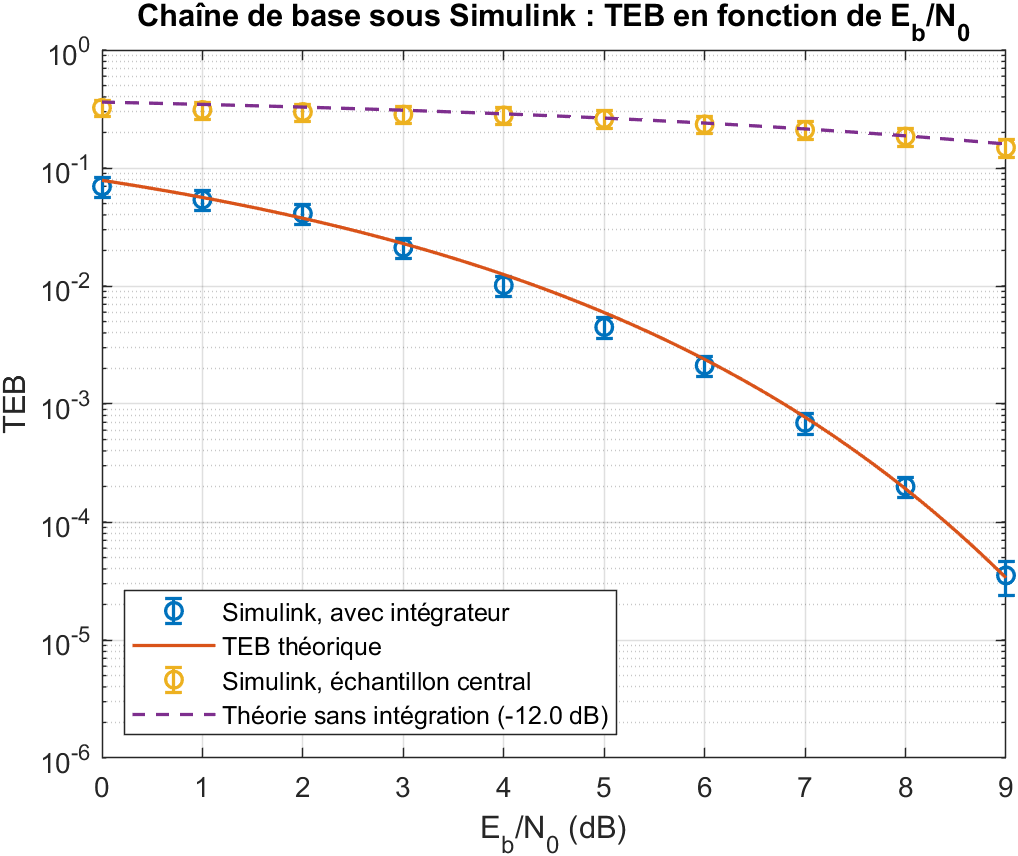
\includegraphics[width=0.55\linewidth]{partie3_simulink_1.png}
\caption{Chaîne de base sous Simulink : TEB avec et sans intégrateur, et courbes théoriques.}
\label{fig:p3}
\end{figure}

% =============================================================================
\section{Codage de canal : code de Hamming C(7,4)}
% =============================================================================
\subsection{Construction du code}
Le code cyclique de polynôme générateur $g(x) = 1 + x + x^3$ est mis sous forme systématique $c = [m_0\,m_1\,m_2\,m_3 \mid r_0\,r_1\,r_2]$ avec $r(x) = x^3m(x) \bmod g(x)$. Les restes des messages de poids 1, $x^3 \equiv 1+x$, $x^4 \equiv x+x^2$, $x^5 \equiv 1+x+x^2$ et $x^6 \equiv 1+x^2$, donnent les lignes de $P$ :
\[
  G = [\,I_4 \mid P\,] = \begin{pmatrix}1&0&0&0&1&1&0\\0&1&0&0&0&1&1\\0&0&1&0&1&1&1\\0&0&0&1&1&0&1\end{pmatrix},
  \qquad
  H = [\,P^T \mid I_3\,] = \begin{pmatrix}1&0&1&1&1&0&0\\1&1&1&0&0&1&0\\0&1&1&1&0&0&1\end{pmatrix}.
\]
On vérifie $GH^T = 0$. Les 7 colonnes de $H$ sont \textbf{non nulles et toutes distinctes} (ce sont les 7 vecteurs non nuls de $\{0,1\}^3$) : aucune combinaison d'une ou deux colonnes n'est nulle, mais il en existe de trois, donc $d_{\min} = 3$ (confirmé par la distribution des poids : 1, 7, 7, 1 mots de poids 0, 3, 4, 7). Le code \textbf{détecte 2 erreurs et en corrige 1}. C'est un code de Hamming car $n = 2^m - 1$ et $k = n - m$ avec $m = 3$ : il est \textbf{parfait}, les $2^3 = 8$ syndromes correspondant exactement aux 8 motifs «~aucune erreur ou une erreur~».

\textbf{Décodage par syndrome.} $s = rH^T$ ; si $s = 0$ le mot est accepté, sinon $s$ est égal à la colonne de $H$ de la position erronée, que l'on inverse. Les fonctions \code{hamming\_enc}/\code{hamming\_dec} (produits matriciels modulo 2) corrigent les 16 messages $\times$ 7 positions d'erreur simple. Avec deux erreurs, le syndrome désigne une troisième position : le décodeur «~corrige~» à tort et produit \textbf{3 bits faux} sur 7.

\subsection{Réalisation sous Simulink par registre à décalage}
Le codeur (\code{codeur\_hamming.slx}, fig.~\ref{fig:lfsr}) n'utilise que 3 \bloc{Unit Delay}, des portes XOR/AND et un \bloc{Switch}, piloté par un compteur de phase modulo 7 : pendant 4 coups d'horloge, le message sort tel quel ($m_3$ en premier) et entre dans le registre diviseur par $g(x)$ ($f = e \oplus s_2$ ; $s_2 \leftarrow s_1$, $s_1 \leftarrow s_0 \oplus f$, $s_0 \leftarrow f$) ; pendant les 3 coups suivants, une porte AND coupe la rétroaction et le \bloc{Switch} bascule sur $s_2$ : le registre se vide et fournit la redondance. Pour $m = [1\,0\,1\,1]$, les états successifs $(s_0 s_1 s_2)$ sont 110, 101, 100, 100 : on obtient $r = [1\,0\,0]$ et le mot \textbf{1011100}, identique au codeur matriciel ; il en va de même pour les 16 messages. Le décodeur (\code{decodeur\_hamming.slx}) présente les 7 bits d'une trame en parallèle grâce à une ligne à retard (\bloc{Tapped Delay}) ; au 7\textsuperscript{e} coup, trois XOR calculent le syndrome $S = 4s_1 + 2s_2 + s_3$, et chaque bit du message est inversé si $S$ vaut le numéro de sa colonne dans $H$ (blocs \bloc{Compare To Constant} + XOR). Testé sur 144 trames (16 messages $\times$ \{0 erreur, 7 erreurs simples\} + double erreur), il est identique au décodeur matriciel de référence.

\begin{figure}[!htb]
\centering
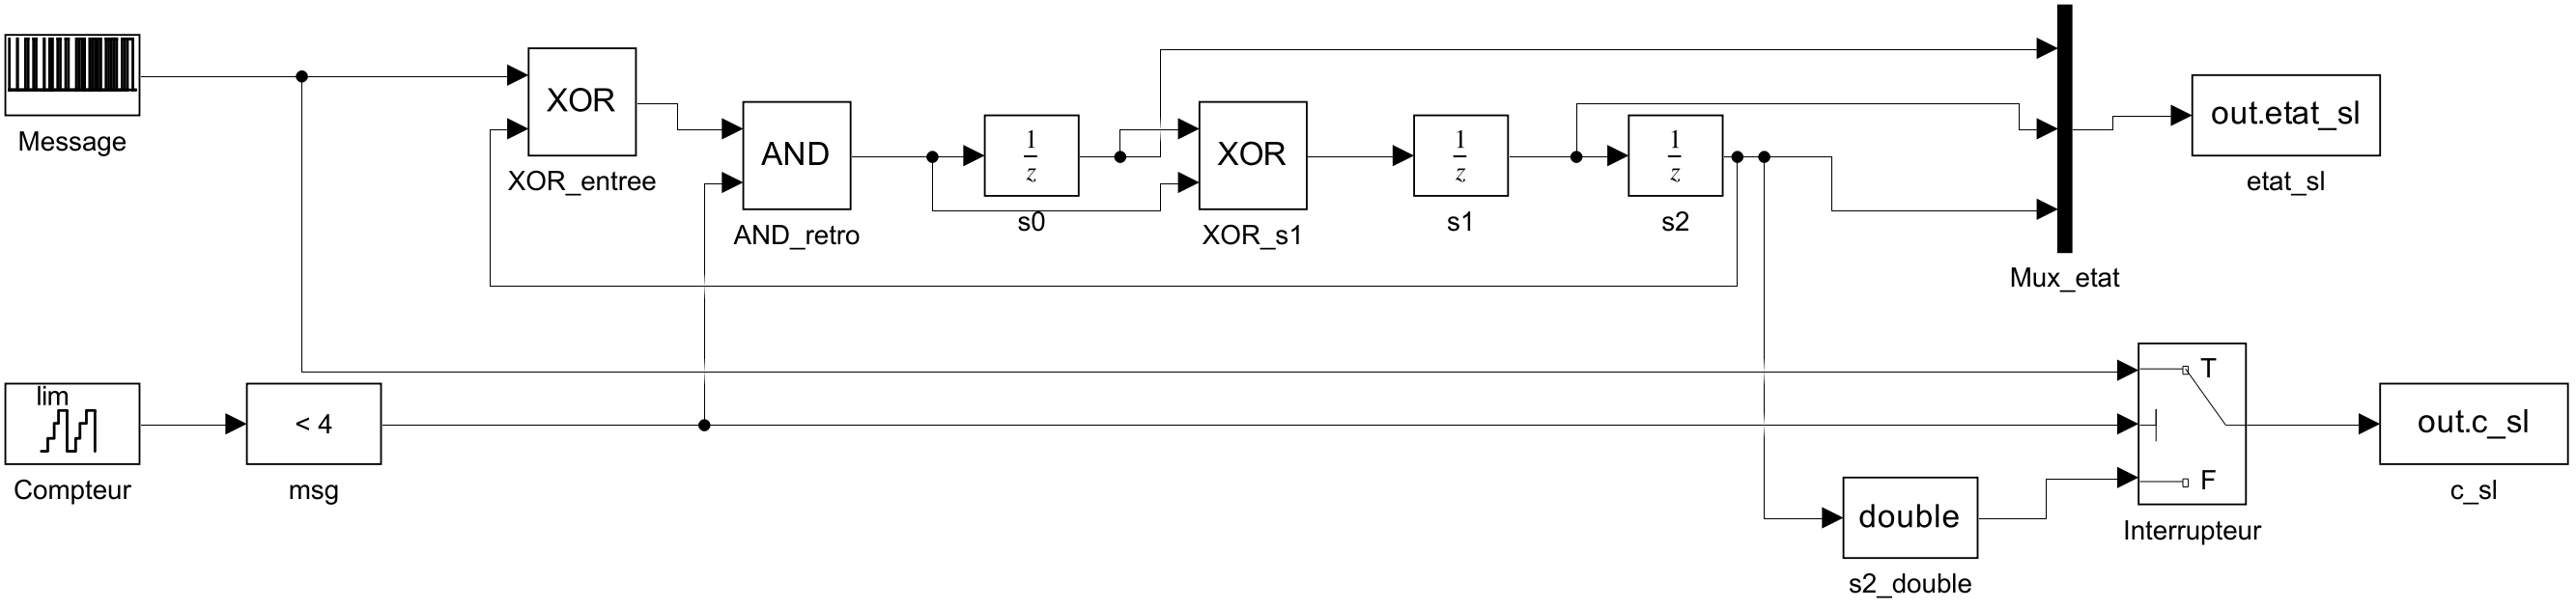
\includegraphics[width=0.85\linewidth]{codeur_hamming.png}
\caption{Codeur de Hamming (7,4) à registre à décalage sous Simulink (\code{codeur\_hamming.slx}).}
\label{fig:lfsr}
\end{figure}

\subsection{Performances théoriques}
Avec $p$ la probabilité d'erreur d'un bit codé, un bloc de 4 bits est juste avec la probabilité $(1-p_0)^4$ sans codage, et $(1-p)^7 + 7p(1-p)^6$ avec codage (0 ou 1 erreur sur 7). À \textbf{$E_b$ fixée}, chaque bit codé ne reçoit que $E_c = \frac47E_b$, d'où $p = Q\big(\sqrt{2\cdot\frac47\,\EbNo}\big)$. Comparer à variance de bruit égale, sans tenir compte du rendement, reviendrait à donner gratuitement 7/4 fois plus d'énergie par bit utile : on surestimerait le gain de $10\log_{10}(7/4) = 2,43$~dB.

L'approximation $P_b \approx \sum_{j\ge2}\frac{j}{7}\binom7j p^j(1-p)^{7-j}$ suppose qu'un mot à $j$ erreurs en garde $j$. Elle est \textbf{optimiste} : un mot à 2 erreurs en contient 3 après «~correction~». Le calcul exact, par énumération des 128 motifs d'erreur, donne $P_b = \sum_w A_w\,p^w(1-p)^{7-w}$ avec $A_w = (0,0,9,19,16,12,7,1)$ : pour $w = 2$, $9/21 = 3/7$ et non $2/7$.

\subsection{Insertion dans la chaîne et gain de codage}
Dans \code{chaine\_P4.slx}, un \bloc{Buffer} de 4 bits alimente le codeur (réalisé sous forme vectorielle, $c = G^Tm \bmod 2$, équivalent au registre validé ; le décodeur reprend la logique du décodeur de la section~4.2). Les bits codés sont émis au rythme $7/(4T_b)$ avec l'amplitude $A\sqrt{4/7}$ (conservation de $E_b$), puis décodés après un \bloc{Buffer} de 7. La difficulté principale est le \textbf{cadrage} : le \bloc{Buffer} de réception doit couper les trames exactement au début des mots-codes. Le script mesure d'abord le retard sur les bits codés (2 bits) et insère un retard d'alignement $K_7 = 5$ pour obtenir un multiple de 7 ; le retard total sur les bits d'information vaut alors $D_4 = 12$ bits.

\begin{figure}[!htb]
\centering
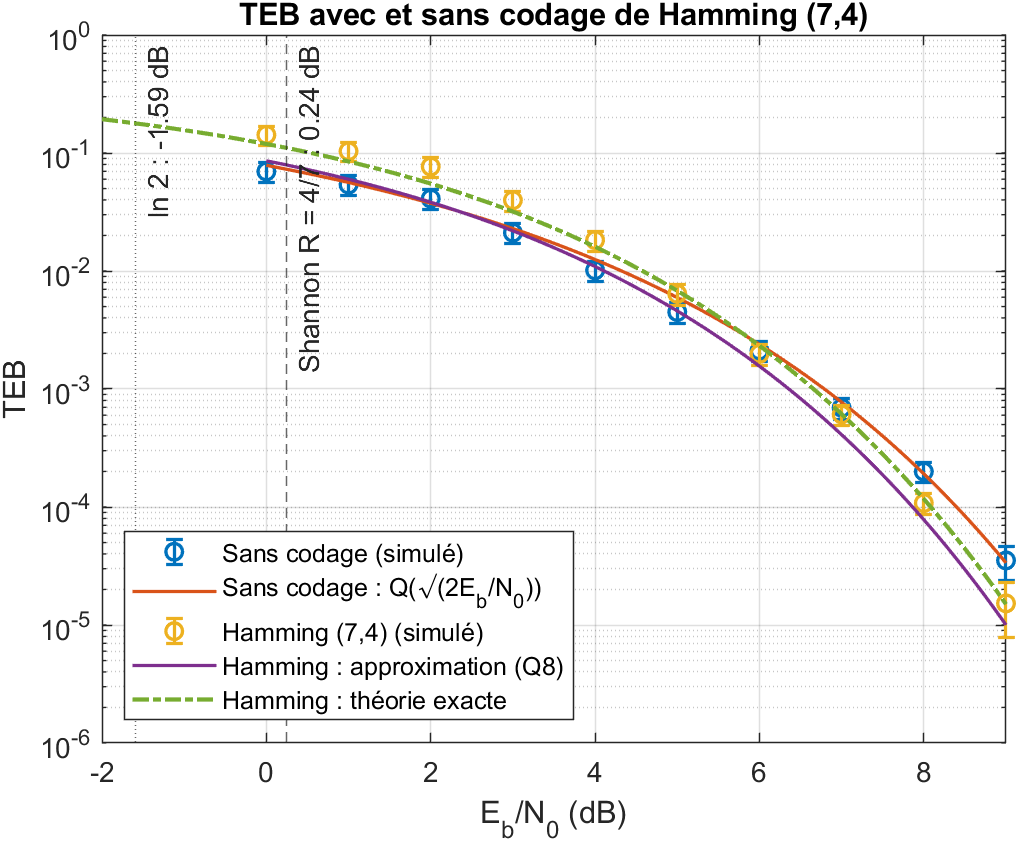
\includegraphics[width=0.6\linewidth]{partie4_chaine_1.png}
\caption{TEB avec et sans code de Hamming (7,4) : simulation, approximation, théorie exacte et limites de Shannon.}
\label{fig:p4}
\end{figure}

La figure~\ref{fig:p4} montre un très bon accord entre la simulation et la \textbf{théorie exacte} (l'approximation est trop optimiste à faible $\EbNo$). À faible rapport signal à bruit, le codage \textbf{dégrade} le TEB (0,14 contre 0,07 à 0~dB) : la perte d'énergie par bit codé n'est pas compensée par la correction d'une seule erreur sur 7. Il ne devient avantageux qu'à partir de \textbf{5,9~dB} (théorie exacte ; confirmé par la simulation, croisement entre 5 et 6~dB). Le \textbf{gain de codage à TEB $=10^{-4}$ n'est que de 0,3~dB} (8,08~dB contre 8,40~dB), et il augmente lentement avec $\EbNo$ (TEB divisé par 2,3 à 9~dB). On reste à \textbf{7,8~dB de la limite de Shannon} pour $R = 4/7$, $\EbNo \ge (2^{2R}-1)/(2R) = 0,24$~dB (et à 10~dB de la limite absolue $\ln 2 = -1,59$~dB) : un code de longueur 7 à décision ferme est très loin des codes longs (turbo-codes, LDPC), qui s'approchent à moins de 1~dB de la limite.

\textbf{Latence et débit.} En temps réel, le codeur systématique émet le message immédiatement, mais doit l'avoir reçu en entier avant de sortir la redondance, et le décodeur doit recevoir les 7 bits avant de corriger : la latence est d'au moins un bloc, environ $2 \times 4T_b$ (12~$T_b$ mesurés dans notre chaîne avec les \bloc{Buffer}). À débit utile constant, le débit binaire du canal est multiplié par \textbf{7/4}, et la bande occupée aussi.

% =============================================================================
\section{Modulation QPSK}
% =============================================================================
\subsection{Mapping de Gray et réalisation}
Chaque couple $(b_1,b_2)$ est associé à un symbole $e^{jk\pi/4}$, $k \in \{1,3,5,7\}$, avec le mapping de Gray \textbf{00 $\to$ $k=1$, 10 $\to$ 3, 11 $\to$ 5, 01 $\to$ 7} : deux symboles voisins ne diffèrent que d'un bit. On a alors $I = (1-2b_1)/\sqrt2$ et $Q = (1-2b_2)/\sqrt2$ : chaque voie porte un bit, indépendamment de l'autre, et la QPSK de Gray équivaut à \textbf{deux BPSK en quadrature}. Avec $E_s = |s|^2 = 1$ et 2 bits par symbole, $E_b = E_s/2 = 1/2$. Le modèle \code{chaine\_P5.slx} (1 échantillon par symbole, $T_s = 2T_b$) groupe les bits par un \bloc{Buffer} de 2 et les envoie sur des tables de correspondance (le mapping est entièrement défini par 4 tables du script, ce qui permet de passer de Gray à naturel sans modifier le modèle). Il ajoute un bruit complexe de variance $N_0/2$ par voie, décide sur le \textbf{signe de chaque voie}, puis démappe et sérialise (\bloc{Unbuffer}). Sans bruit, on obtient 0 erreur avec un retard $D_5 = 2$ bits.

\begin{figure}[!htb]
\centering
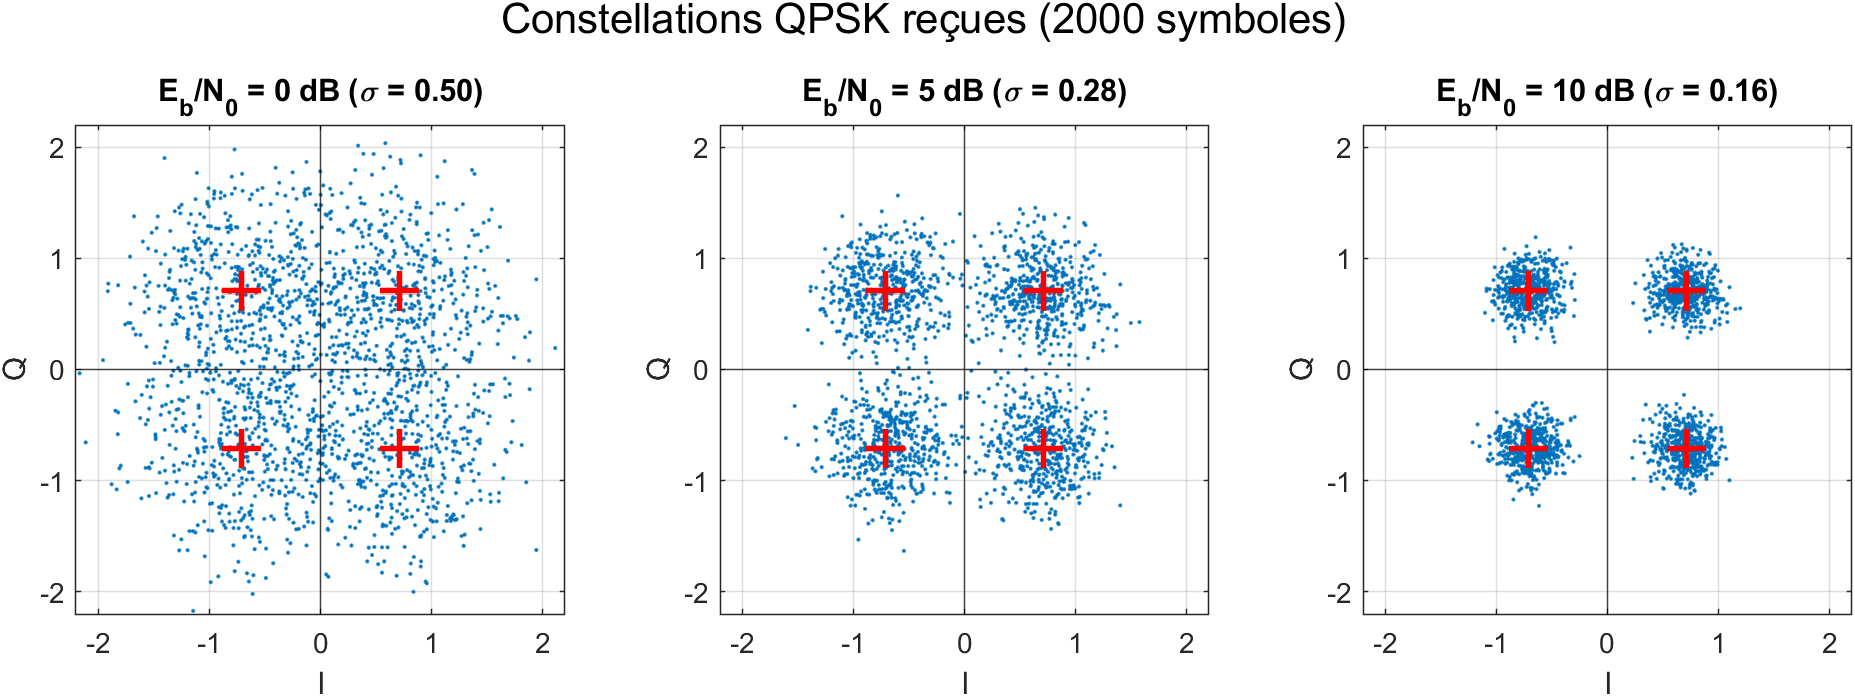
\includegraphics[width=0.92\linewidth]{partie5_qpsk_1.png}
\caption{Constellations QPSK reçues à $\EbNo$ = 0, 5 et 10~dB (2\,000 symboles).}
\label{fig:const}
\end{figure}

\textbf{Constellations (fig.~\ref{fig:const}).} Les nuages sont centrés sur les 4 symboles, avec un écart-type par voie $\sigma = \sqrt{N_0/2}$ = 0,50, 0,28 et 0,16. À 0~dB, les nuages débordent largement sur les quadrants voisins (TEB $\approx$ 8\,\%) ; à 10~dB, ils sont parfaitement séparés (TEB $\approx 4\cdot10^{-6}$). Les erreurs se font presque toujours vers un \textbf{symbole adjacent}, d'où l'intérêt du mapping de Gray.

\begin{figure}[!htb]
\centering
\begin{subfigure}{0.49\linewidth}\centering
  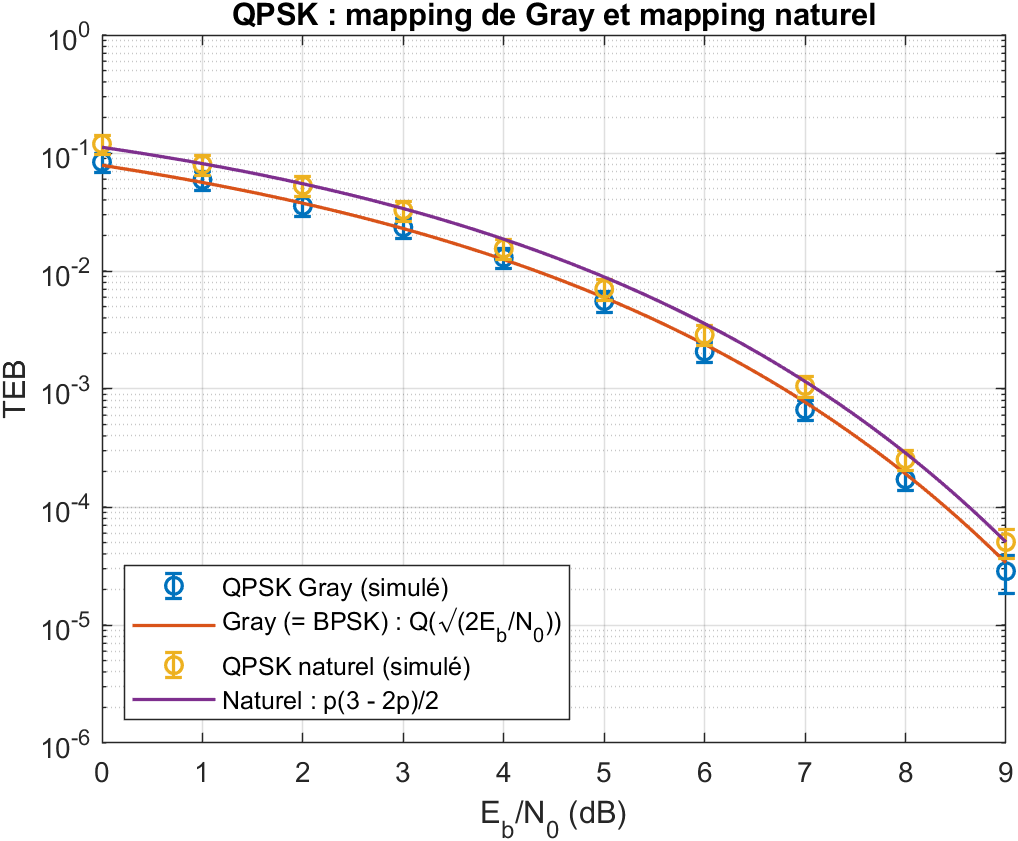
\includegraphics[width=\linewidth]{partie5_qpsk_2.png}
  \caption{Mapping de Gray et mapping naturel.}
\end{subfigure}\hfill
\begin{subfigure}{0.49\linewidth}\centering
  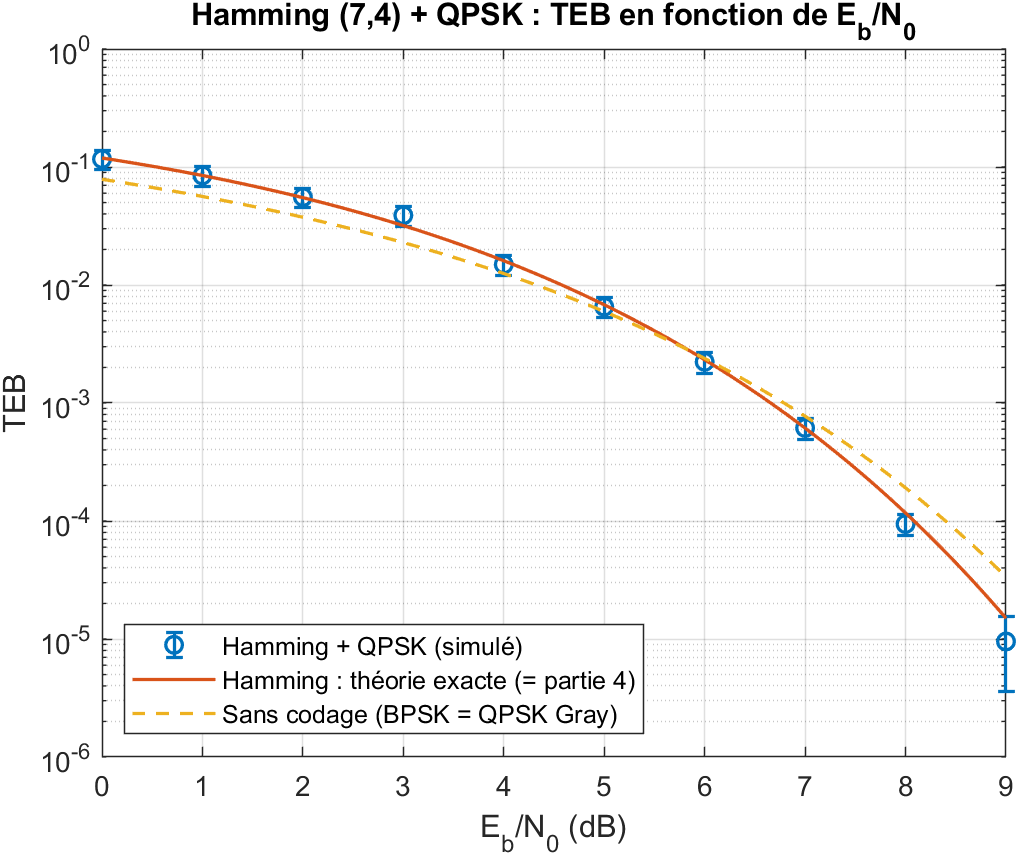
\includegraphics[width=\linewidth]{partie5_q6_1.png}
  \caption{Hamming (7,4) + QPSK de Gray.}
\end{subfigure}
\caption{TEB des chaînes QPSK : simulation et théorie.}
\label{fig:qpsk}
\end{figure}

\subsection{Performances et comparaison avec la chaîne binaire}
Avec Gray, le TEB simulé suit exactement $Q(\sqrt{2\EbNo})$ (fig.~\ref{fig:qpsk}a) : \textbf{à $\EbNo$ égal, la QPSK a le même TEB que la transmission binaire antipodale} de la partie~3. En revanche, \textbf{à durée de symbole égale, elle transmet deux fois plus de bits}, et \textbf{à débit binaire égal, elle occupe deux fois moins de bande} ($T_s = 2T_b$). C'est un gain gratuit en efficacité spectrale, obtenu parce que les voies I et Q sont orthogonales.

\textbf{Mapping naturel} (00, 01, 10, 11 $\to$ $k$ = 1, 3, 5, 7). Les symboles 01 ($k=3$) et 10 ($k=5$), voisins, diffèrent de 2 bits, de même que 11 et 00. Avec $p = Q(\sqrt{2\EbNo})$ par voie, on montre que $\TEB = p(3-2p)/2 \approx 1,5\,p$ : une erreur vers un voisin coûte en moyenne 1,5 bit au lieu de 1. La simulation suit cette expression ; la perte vaut \textbf{0,23~dB à TEB $=10^{-4}$} (8,63~dB contre 8,40~dB). Elle est faible en dB, car le TEB décroît très vite, mais systématique.

\subsection{Chaîne codée Hamming + QPSK}
Un mot-code a 7 bits, nombre impair : grouper les bits par paires mot par mot imposerait du bourrage. On sérialise donc les mots-codes (\bloc{Unbuffer}, rythme $T_c = 4T_b/7$), puis on regroupe le \textbf{flux continu} de bits codés par un \bloc{Buffer} de 2 : un symbole QPSK dure $T_{s,c} = 2T_c = 8T_b/7$, et un mot-code sur deux commence au milieu d'un symbole. Cela ne pose aucun problème, puisque le récepteur re-sérialise les bits avant de recouper les mots (retard d'alignement $K_7 = 5$, retard total 12 bits). Comme les deux voies de la QPSK de Gray sont des BPSK indépendantes d'énergie $E_c = \frac47E_b$ par bit codé, le TEB est \textbf{identique à celui de la partie~4} (fig.~\ref{fig:qpsk}b : simulation conforme à la théorie exacte, $9,4\cdot10^{-5}$ à 8~dB), mais la bande est divisée par 2 : \textbf{7/8 de la bande de la chaîne binaire non codée}, au lieu de 7/4. La QPSK compense ainsi l'expansion de bande due au codage.

% =============================================================================
\section{Filtre de mise en forme et filtre adapté}
% =============================================================================
Le modèle \code{chaine\_P6.slx} revient à $L = 16$ échantillons par symbole : les symboles QPSK sont placés tous les $L$ échantillons, filtrés par $h$ (bloc \bloc{Discrete FIR Filter}), bruités, filtrés par le filtre adapté $h(-t)$, puis échantillonnés une fois par symbole. Les filtres sont normalisés à énergie unité : le bruit après filtre adapté garde la variance $\sigma^2$ par voie et l'échantillon optimal vaut le symbole émis. Les retards sont, là encore, déterminés automatiquement : $D_7 = 6$ bits avec la porte, \textbf{24 bits} avec le RRC, dont 10 symboles (20 bits) dus aux deux filtres de $N = 10L+1 = 161$ coefficients.

\subsection{Filtre porte}
Avec $h$ égal à une porte de durée $T$, le filtre adapté est la même porte, et la sortie échantillonnée à la fin du symbole vaut $\int_{kT}^{(k+1)T} r(t)\,dt$ à un facteur près : c'est \textbf{exactement l'intégrateur à remise à zéro de la figure~\ref{fig:p3}}. Le TEB est bien inchangé et suit $Q(\sqrt{2\EbNo})$ (fig.~\ref{fig:p6teb}a). L'œil est triangulaire, complètement ouvert au seul instant optimal.

\subsection{Racine de cosinus surélevé ($\alpha = 0,35$)}
La fonction \code{rrc\_coef} calcule $h$ en traitant les deux points singuliers par leurs limites :
\[
  h(0) = \frac{1}{\sqrt T}\Big(1-\alpha+\frac{4\alpha}{\pi}\Big) = 1,0956,
  \qquad
  h\Big(\pm\frac{T}{4\alpha}\Big) = \frac{\alpha}{\sqrt{2T}}\Big[\Big(1+\frac2\pi\Big)\sin\frac{\pi}{4\alpha} + \Big(1-\frac2\pi\Big)\cos\frac{\pi}{4\alpha}\Big] = 0,2606,
\]
la continuité étant vérifiée numériquement. Les coefficients normalisés coïncident avec \code{rcosdesign} à $4\cdot10^{-16}$ près.

\begin{figure}[!htb]
\centering
\begin{subfigure}{0.64\linewidth}\centering
  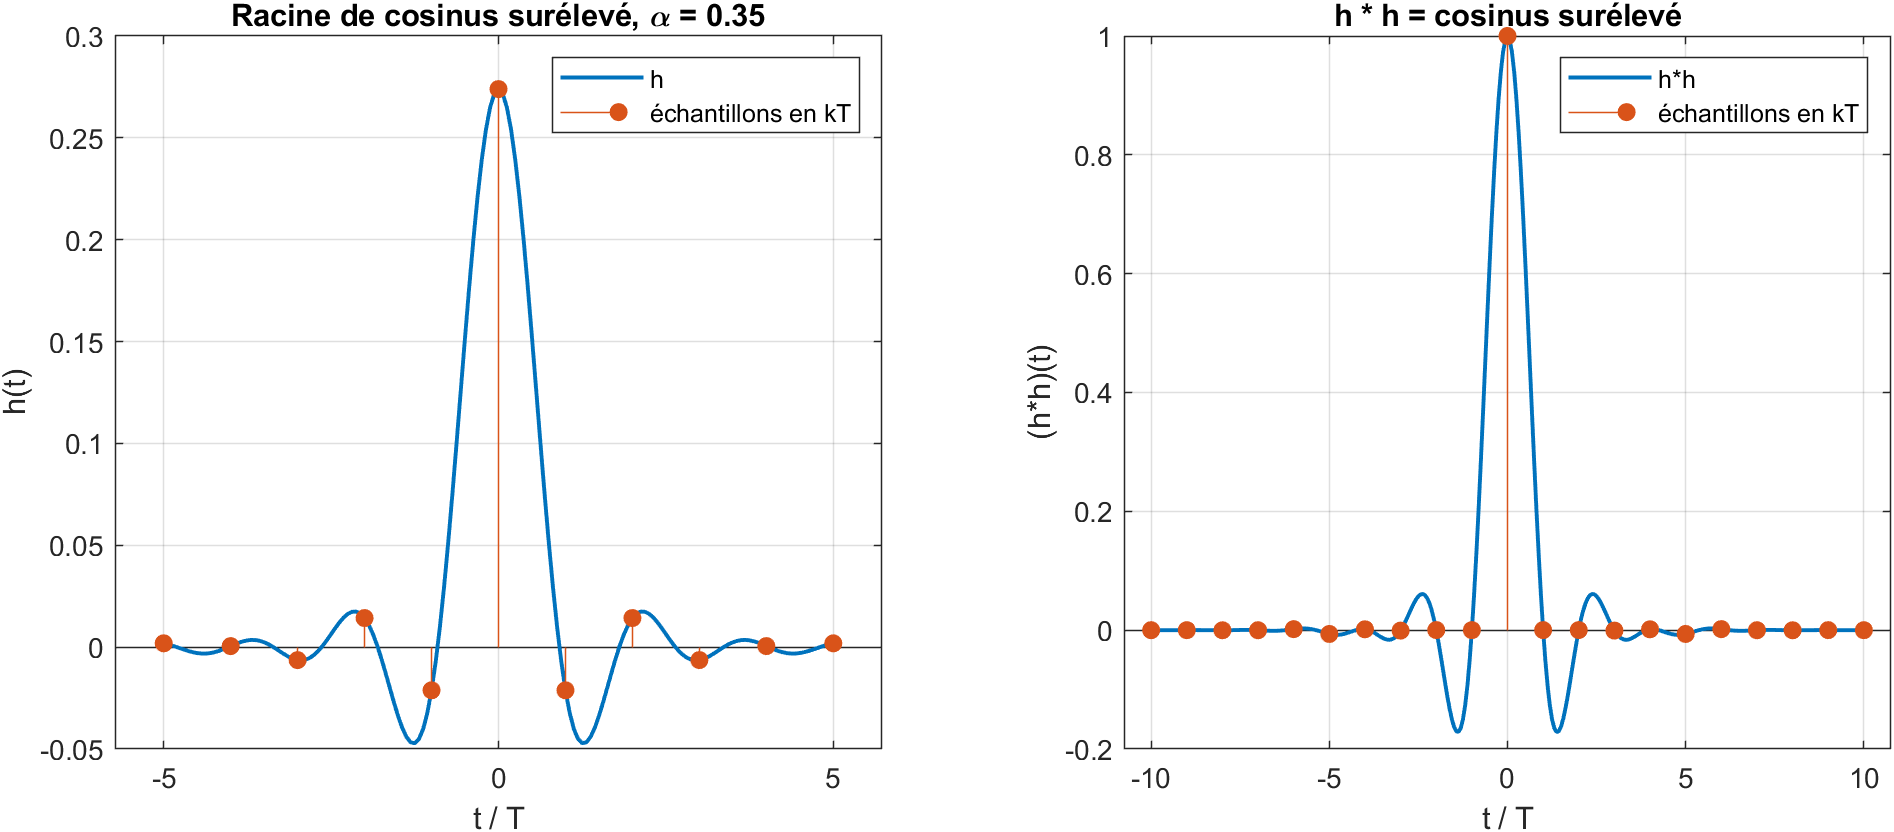
\includegraphics[width=\linewidth]{partie6_filtres_1.png}
  \caption{$h$ (RRC) et $h*h$ (cosinus surélevé), échantillons en $kT$.}
\end{subfigure}\hfill
\begin{subfigure}{0.34\linewidth}\centering
  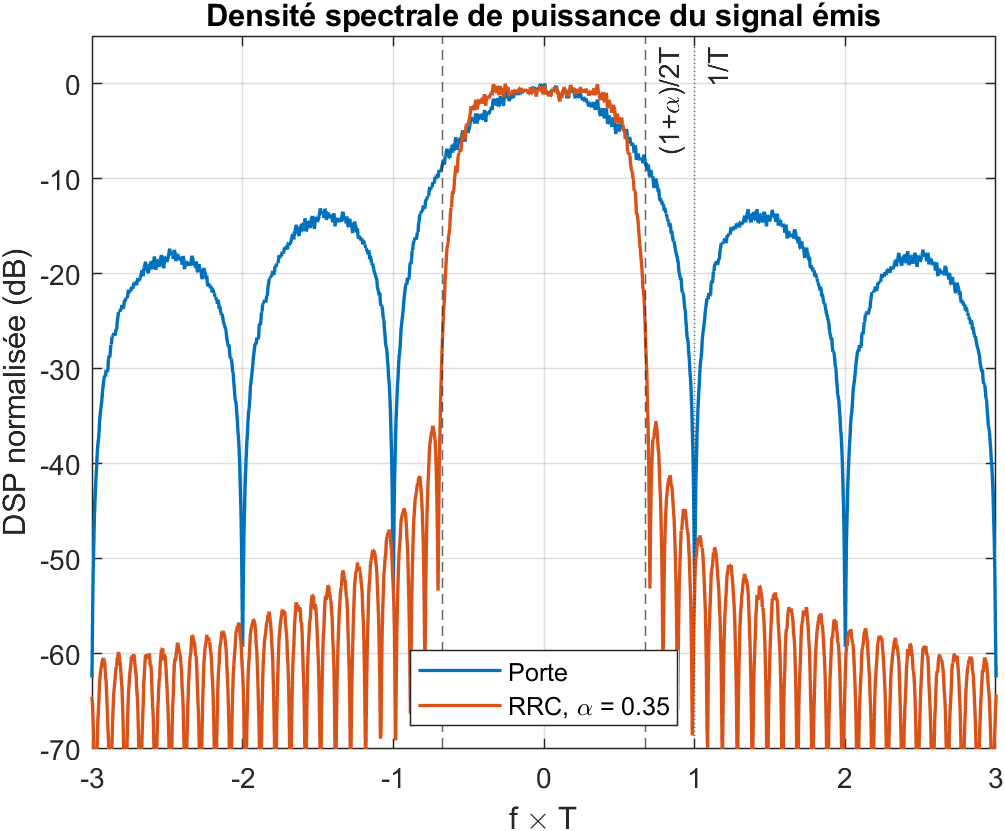
\includegraphics[width=\linewidth]{partie6_filtres_2.png}
  \caption{DSP du signal émis.}
\end{subfigure}
\caption{Filtre en racine de cosinus surélevé ($\alpha = 0,35$, troncature à 10 symboles).}
\label{fig:rrc}
\end{figure}

\textbf{Critère de Nyquist (fig.~\ref{fig:rrc}a).} $h$ seul ne s'annule pas aux multiples de $T$ (jusqu'à $2,1\cdot10^{-2}$) : c'est le \textbf{produit $h*h$}, un cosinus surélevé, qui vérifie $g(kT) = \delta_k$. L'IES n'est donc nulle \textbf{qu'après le filtre adapté, aux instants d'échantillonnage} ; le partage «~racine~» entre émission et réception réalise en même temps le filtrage adapté. La troncature à 10 symboles laisse une IES résiduelle de $6,4\cdot10^{-3}$ ($5\cdot10^{-2}$ pour 4 symboles, $7\cdot10^{-4}$ pour 24) et des lobes secondaires vers $-40$~dB dans le spectre.

\textbf{Spectre (fig.~\ref{fig:rrc}b).} Avec la porte, la DSP est en $\mathrm{sinc}^2$, avec des lobes secondaires à $-13$~dB qui décroissent lentement : 99\,\% de la puissance tient dans \textbf{5,56/$T$}. Avec le RRC, la DSP est confinée à $|f| \le (1+\alpha)/(2T) = 0,675/T$, et 99\,\% de la puissance tient dans \textbf{0,58/$T$} (la zone de retombée porte peu de puissance) : la bande est divisée par \textbf{9,6}.

\begin{figure}[!htb]
\centering
\begin{subfigure}{0.49\linewidth}\centering
  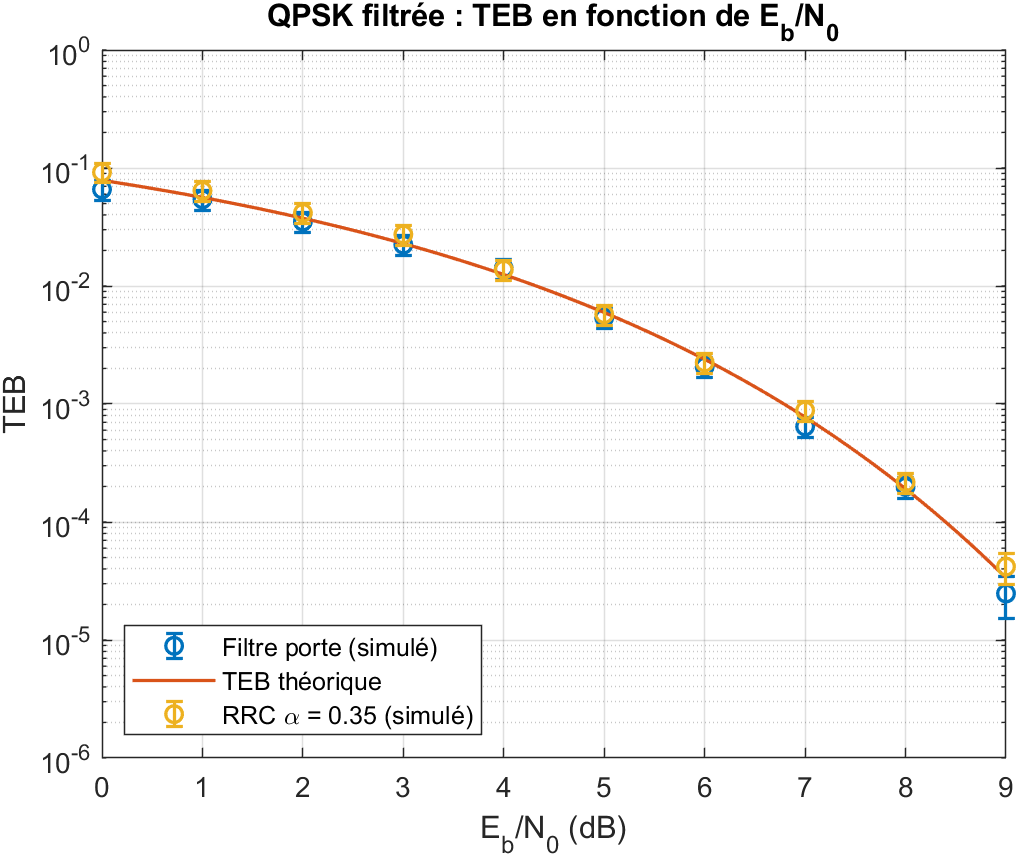
\includegraphics[width=\linewidth]{partie6_chaine_1.png}
  \caption{Filtre porte et filtre RRC.}
\end{subfigure}\hfill
\begin{subfigure}{0.49\linewidth}\centering
  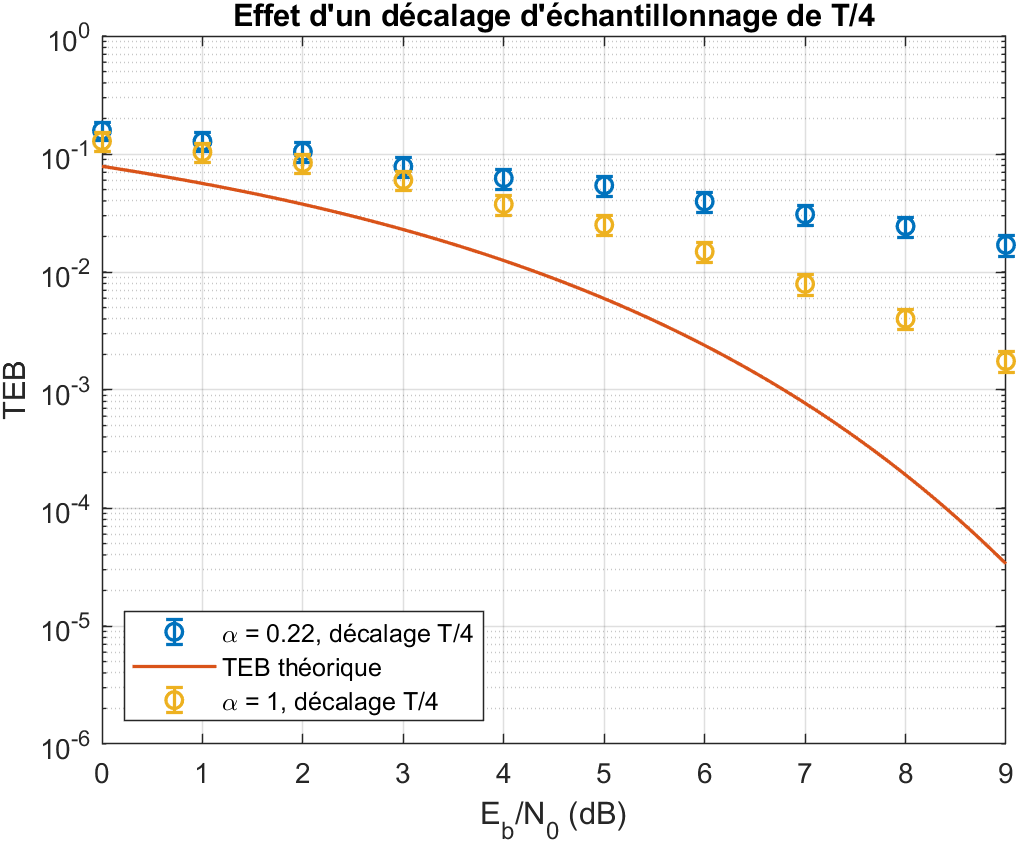
\includegraphics[width=\linewidth]{partie6_chaine_4.png}
  \caption{Décalage d'échantillonnage de $T/4$.}
\end{subfigure}
\caption{TEB de la chaîne QPSK filtrée.}
\label{fig:p6teb}
\end{figure}

\textbf{Insertion dans la chaîne.} Le diagramme de l'œil sans bruit (fig.~\ref{fig:oeil}) montre que toutes les trajectoires passent par $\pm1/\sqrt2$ à l'instant optimal : l'œil est parfaitement ouvert à $t = 0$, malgré des dépassements jusqu'à $\pm1,1$ entre les instants de décision. Les constellations à 10~dB sont identiques à celles de la partie~5 (les quelques points près de l'origine correspondent au remplissage des filtres en début de simulation). Le TEB avec RRC suit la théorie jusqu'à 7~dB, avec une légère dégradation à fort $\EbNo$ ($2,2\cdot10^{-4}$ contre $1,9\cdot10^{-4}$ à 8~dB, soit environ 0,1~dB), imputable à l'IES résiduelle de troncature. Le \textbf{débit} est celui de la partie~5 (2 bits par symbole), mais dans une bande \textbf{strictement limitée} à $(1+\alpha)/(2T_s)$, soit une efficacité spectrale d'environ 1,5~bit/s/Hz.

\begin{figure}[!htb]
\centering
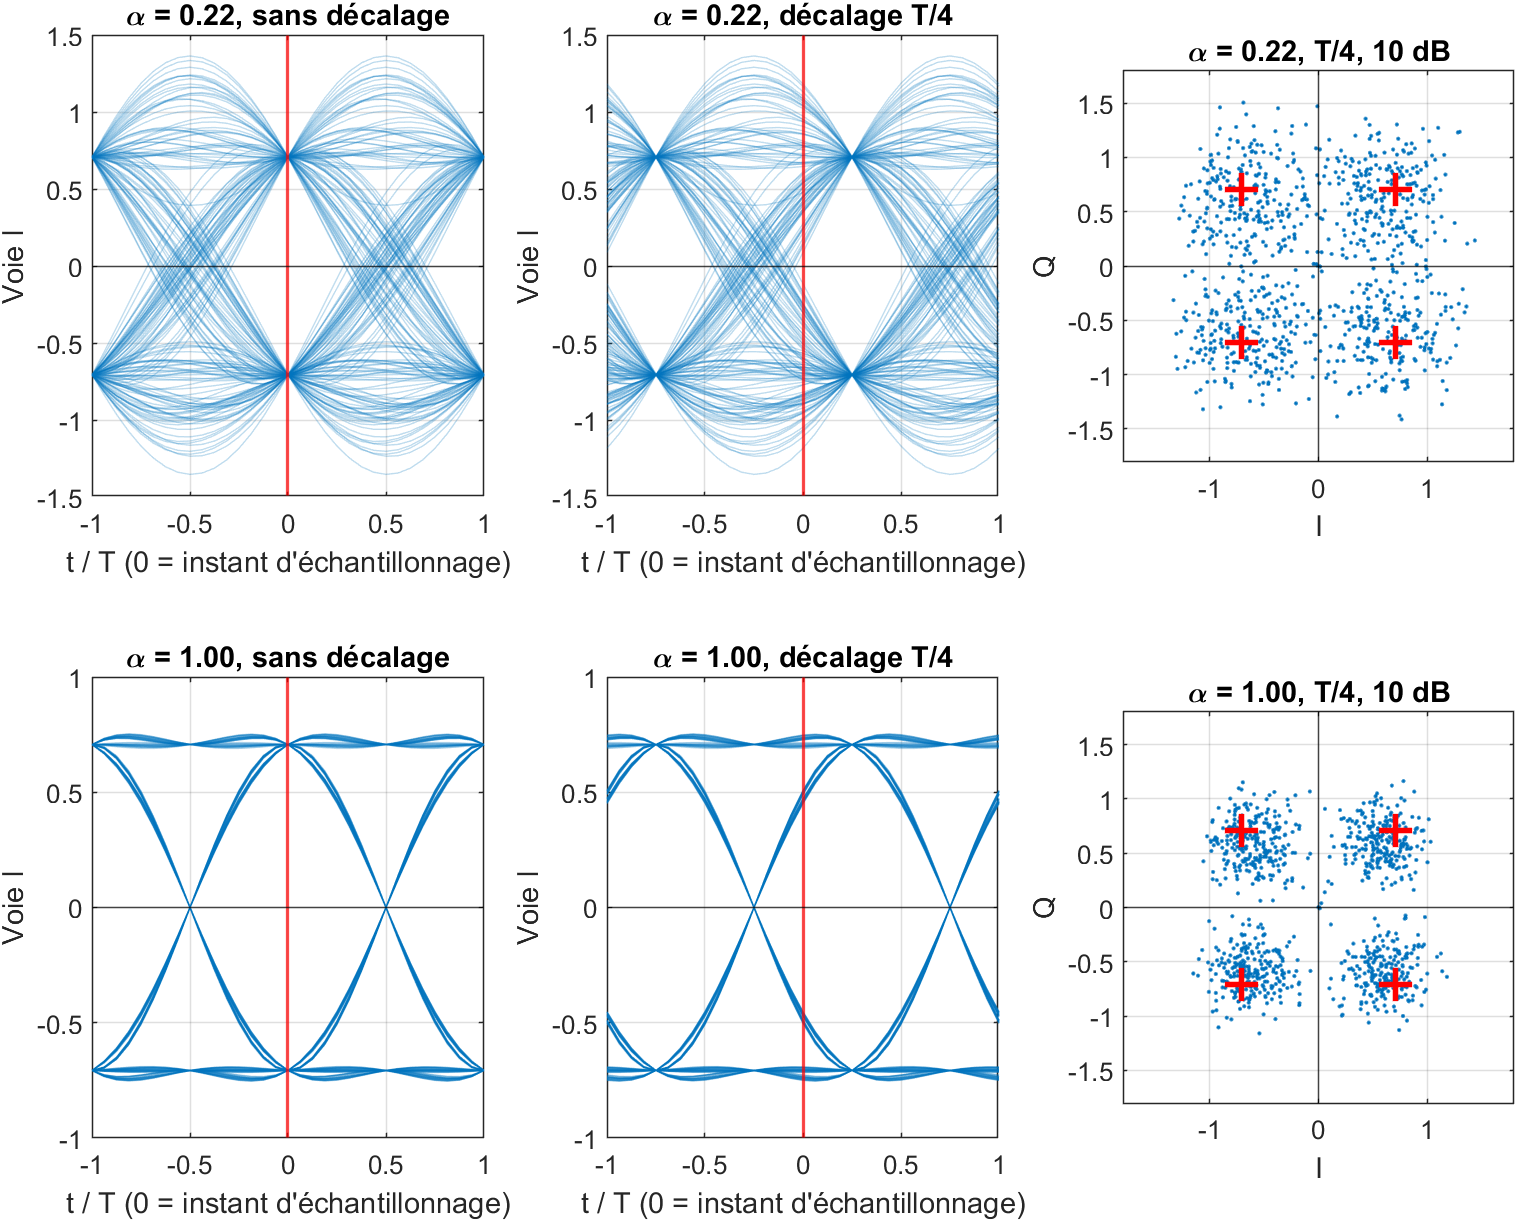
\includegraphics[width=0.8\linewidth]{partie6_chaine_3.png}
\caption{Diagrammes de l'œil sans bruit (sans et avec décalage $T/4$) et constellations à 10~dB avec décalage : $\alpha = 0,22$ (haut) et $\alpha = 1$ (bas).}
\label{fig:oeil}
\end{figure}

\textbf{Décalage de l'instant d'échantillonnage de $T/4$ (fig.~\ref{fig:p6teb}b et~\ref{fig:oeil}).} Pour $\alpha = 0,22$, l'œil est étroit : à $T/4$ de l'instant optimal, les trajectoires sont très dispersées, la constellation s'étale en nuages diffus et le TEB est multiplié par 17 à 6~dB ($3,96\cdot10^{-2}$ contre $2,39\cdot10^{-3}$). Il plafonne vers $2\cdot10^{-2}$ à 9~dB, car l'IES, indépendante du bruit, impose un plancher d'erreurs. Pour $\alpha = 1$, les queues de $h$ décroissent beaucoup plus vite, l'œil est large et les trajectoires restent groupées : la perte se réduit pour l'essentiel à une baisse d'amplitude utile ($1,5\cdot10^{-2}$ à 6~dB, $1,8\cdot10^{-3}$ à 9~dB). On retrouve le \textbf{compromis entre bande et robustesse à la synchronisation} : un faible roll-off économise de la bande ($0,61/T$ contre $1/T$), mais il exige une récupération de rythme précise.

% =============================================================================
\section{Conclusion}
% =============================================================================
\begin{table}[!htb]
\centering\small
\begin{tabular}{>{\raggedright}p{0.24\linewidth} >{\raggedright}p{0.36\linewidth} >{\raggedright\arraybackslash}p{0.33\linewidth}}
\toprule
\textbf{Bloc ajouté} & \textbf{Effet sur le TEB} & \textbf{Débit / bande (débit utile fixé)} \\
\midrule
Codage de source & --- & 7 $\to$ 4,58 bit/car. (Huffman), 2,51 (bzip2) \\
Détecteur optimal (intégrateur) & +12~dB par rapport à 1 échantillon/bit ; $10^{-4}$ à 8,4~dB & inchangés \\
Hamming (7,4) & perte sous 5,9~dB ; gain de 0,3~dB à $10^{-4}$ & débit canal et bande $\times$ 7/4 ; latence $\approx$ 1 bloc \\
QPSK (Gray) & inchangé ($-0,23$~dB en mapping naturel) & bande $\div$ 2 \\
Mise en forme RRC ($\alpha = 0,35$) & inchangé ($\approx$ 0,1~dB de troncature) ; sensible au rythme & bande à 99\,\% : 5,56/$T$ $\to$ 0,58/$T$ \\
\bottomrule
\end{tabular}
\caption{Synthèse de l'apport de chaque bloc.}
\label{tab:synthese}
\end{table}

Ce TP a permis de construire une chaîne complète, validée à chaque étape par la théorie : les courbes de TEB simulées tombent dans leur intervalle de confiance autour des expressions analytiques, ce qui valide à la fois les modèles et la méthode (énergie par bit d'information constante, compensation automatique des retards, 100 erreurs par point). Le codage de source retire la redondance et produit des bits quasi équiprobables, ce qui justifie le modèle de source utilisé ensuite. Côté transmission, ce sont le \textbf{filtrage adapté} (12~dB) et le \textbf{choix de la modulation et de la mise en forme} (bande divisée par 2, puis par près de 10, sans perte de TEB) qui apportent le plus. Le code de Hamming apporte peu : 0,3~dB à $10^{-4}$ pour 75\,\% de bande supplémentaire.

\textbf{Par rapport aux limites de Shannon}, la chaîne non codée atteint $10^{-4}$ à 8,4~dB et la chaîne codée à 8,1~dB, alors qu'une transmission fiable est possible dès 0,24~dB au rendement 4/7 ($-1,59$~dB à rendement nul) : il reste \textbf{près de 8~dB} à gagner, que seuls des codes longs à décodage souple (convolutifs, turbo-codes, LDPC) permettent d'approcher. La partie~7 (canal à deux trajets, $\beta = 0,23$, $\tau = 2T$), non traitée, constituerait la suite naturelle : l'écho rompt le critère de Nyquist de la chaîne et impose un égaliseur (forçage à zéro ou MMSE), qui nécessite d'estimer la réponse du canal, par exemple à l'aide d'une séquence d'apprentissage.

\end{document}
